% Options for packages loaded elsewhere
\PassOptionsToPackage{unicode}{hyperref}
\PassOptionsToPackage{hyphens}{url}
\PassOptionsToPackage{dvipsnames,svgnames,x11names}{xcolor}
%
\documentclass[
  letterpaper,
  DIV=11,
  numbers=noendperiod]{scrartcl}

\usepackage{amsmath,amssymb}
\usepackage{iftex}
\ifPDFTeX
  \usepackage[T1]{fontenc}
  \usepackage[utf8]{inputenc}
  \usepackage{textcomp} % provide euro and other symbols
\else % if luatex or xetex
  \usepackage{unicode-math}
  \defaultfontfeatures{Scale=MatchLowercase}
  \defaultfontfeatures[\rmfamily]{Ligatures=TeX,Scale=1}
\fi
\usepackage{lmodern}
\ifPDFTeX\else  
    % xetex/luatex font selection
\fi
% Use upquote if available, for straight quotes in verbatim environments
\IfFileExists{upquote.sty}{\usepackage{upquote}}{}
\IfFileExists{microtype.sty}{% use microtype if available
  \usepackage[]{microtype}
  \UseMicrotypeSet[protrusion]{basicmath} % disable protrusion for tt fonts
}{}
\makeatletter
\@ifundefined{KOMAClassName}{% if non-KOMA class
  \IfFileExists{parskip.sty}{%
    \usepackage{parskip}
  }{% else
    \setlength{\parindent}{0pt}
    \setlength{\parskip}{6pt plus 2pt minus 1pt}}
}{% if KOMA class
  \KOMAoptions{parskip=half}}
\makeatother
\usepackage{xcolor}
\setlength{\emergencystretch}{3em} % prevent overfull lines
\setcounter{secnumdepth}{-\maxdimen} % remove section numbering
% Make \paragraph and \subparagraph free-standing
\makeatletter
\ifx\paragraph\undefined\else
  \let\oldparagraph\paragraph
  \renewcommand{\paragraph}{
    \@ifstar
      \xxxParagraphStar
      \xxxParagraphNoStar
  }
  \newcommand{\xxxParagraphStar}[1]{\oldparagraph*{#1}\mbox{}}
  \newcommand{\xxxParagraphNoStar}[1]{\oldparagraph{#1}\mbox{}}
\fi
\ifx\subparagraph\undefined\else
  \let\oldsubparagraph\subparagraph
  \renewcommand{\subparagraph}{
    \@ifstar
      \xxxSubParagraphStar
      \xxxSubParagraphNoStar
  }
  \newcommand{\xxxSubParagraphStar}[1]{\oldsubparagraph*{#1}\mbox{}}
  \newcommand{\xxxSubParagraphNoStar}[1]{\oldsubparagraph{#1}\mbox{}}
\fi
\makeatother

\usepackage{color}
\usepackage{fancyvrb}
\newcommand{\VerbBar}{|}
\newcommand{\VERB}{\Verb[commandchars=\\\{\}]}
\DefineVerbatimEnvironment{Highlighting}{Verbatim}{commandchars=\\\{\}}
% Add ',fontsize=\small' for more characters per line
\usepackage{framed}
\definecolor{shadecolor}{RGB}{241,243,245}
\newenvironment{Shaded}{\begin{snugshade}}{\end{snugshade}}
\newcommand{\AlertTok}[1]{\textcolor[rgb]{0.68,0.00,0.00}{#1}}
\newcommand{\AnnotationTok}[1]{\textcolor[rgb]{0.37,0.37,0.37}{#1}}
\newcommand{\AttributeTok}[1]{\textcolor[rgb]{0.40,0.45,0.13}{#1}}
\newcommand{\BaseNTok}[1]{\textcolor[rgb]{0.68,0.00,0.00}{#1}}
\newcommand{\BuiltInTok}[1]{\textcolor[rgb]{0.00,0.23,0.31}{#1}}
\newcommand{\CharTok}[1]{\textcolor[rgb]{0.13,0.47,0.30}{#1}}
\newcommand{\CommentTok}[1]{\textcolor[rgb]{0.37,0.37,0.37}{#1}}
\newcommand{\CommentVarTok}[1]{\textcolor[rgb]{0.37,0.37,0.37}{\textit{#1}}}
\newcommand{\ConstantTok}[1]{\textcolor[rgb]{0.56,0.35,0.01}{#1}}
\newcommand{\ControlFlowTok}[1]{\textcolor[rgb]{0.00,0.23,0.31}{\textbf{#1}}}
\newcommand{\DataTypeTok}[1]{\textcolor[rgb]{0.68,0.00,0.00}{#1}}
\newcommand{\DecValTok}[1]{\textcolor[rgb]{0.68,0.00,0.00}{#1}}
\newcommand{\DocumentationTok}[1]{\textcolor[rgb]{0.37,0.37,0.37}{\textit{#1}}}
\newcommand{\ErrorTok}[1]{\textcolor[rgb]{0.68,0.00,0.00}{#1}}
\newcommand{\ExtensionTok}[1]{\textcolor[rgb]{0.00,0.23,0.31}{#1}}
\newcommand{\FloatTok}[1]{\textcolor[rgb]{0.68,0.00,0.00}{#1}}
\newcommand{\FunctionTok}[1]{\textcolor[rgb]{0.28,0.35,0.67}{#1}}
\newcommand{\ImportTok}[1]{\textcolor[rgb]{0.00,0.46,0.62}{#1}}
\newcommand{\InformationTok}[1]{\textcolor[rgb]{0.37,0.37,0.37}{#1}}
\newcommand{\KeywordTok}[1]{\textcolor[rgb]{0.00,0.23,0.31}{\textbf{#1}}}
\newcommand{\NormalTok}[1]{\textcolor[rgb]{0.00,0.23,0.31}{#1}}
\newcommand{\OperatorTok}[1]{\textcolor[rgb]{0.37,0.37,0.37}{#1}}
\newcommand{\OtherTok}[1]{\textcolor[rgb]{0.00,0.23,0.31}{#1}}
\newcommand{\PreprocessorTok}[1]{\textcolor[rgb]{0.68,0.00,0.00}{#1}}
\newcommand{\RegionMarkerTok}[1]{\textcolor[rgb]{0.00,0.23,0.31}{#1}}
\newcommand{\SpecialCharTok}[1]{\textcolor[rgb]{0.37,0.37,0.37}{#1}}
\newcommand{\SpecialStringTok}[1]{\textcolor[rgb]{0.13,0.47,0.30}{#1}}
\newcommand{\StringTok}[1]{\textcolor[rgb]{0.13,0.47,0.30}{#1}}
\newcommand{\VariableTok}[1]{\textcolor[rgb]{0.07,0.07,0.07}{#1}}
\newcommand{\VerbatimStringTok}[1]{\textcolor[rgb]{0.13,0.47,0.30}{#1}}
\newcommand{\WarningTok}[1]{\textcolor[rgb]{0.37,0.37,0.37}{\textit{#1}}}

\providecommand{\tightlist}{%
  \setlength{\itemsep}{0pt}\setlength{\parskip}{0pt}}\usepackage{longtable,booktabs,array}
\usepackage{calc} % for calculating minipage widths
% Correct order of tables after \paragraph or \subparagraph
\usepackage{etoolbox}
\makeatletter
\patchcmd\longtable{\par}{\if@noskipsec\mbox{}\fi\par}{}{}
\makeatother
% Allow footnotes in longtable head/foot
\IfFileExists{footnotehyper.sty}{\usepackage{footnotehyper}}{\usepackage{footnote}}
\makesavenoteenv{longtable}
\usepackage{graphicx}
\makeatletter
\newsavebox\pandoc@box
\newcommand*\pandocbounded[1]{% scales image to fit in text height/width
  \sbox\pandoc@box{#1}%
  \Gscale@div\@tempa{\textheight}{\dimexpr\ht\pandoc@box+\dp\pandoc@box\relax}%
  \Gscale@div\@tempb{\linewidth}{\wd\pandoc@box}%
  \ifdim\@tempb\p@<\@tempa\p@\let\@tempa\@tempb\fi% select the smaller of both
  \ifdim\@tempa\p@<\p@\scalebox{\@tempa}{\usebox\pandoc@box}%
  \else\usebox{\pandoc@box}%
  \fi%
}
% Set default figure placement to htbp
\def\fps@figure{htbp}
\makeatother

\KOMAoption{captions}{tableheading}
\usepackage{float}
\floatplacement{table}{H}
\floatplacement{figure}{H}
\newcommand{\legend}[1]{\textcolor{red}{\textbf{\textit{#1}}}}
\makeatletter
\@ifpackageloaded{caption}{}{\usepackage{caption}}
\AtBeginDocument{%
\ifdefined\contentsname
  \renewcommand*\contentsname{Tabla de contenidos}
\else
  \newcommand\contentsname{Tabla de contenidos}
\fi
\ifdefined\listfigurename
  \renewcommand*\listfigurename{Listado de Figuras}
\else
  \newcommand\listfigurename{Listado de Figuras}
\fi
\ifdefined\listtablename
  \renewcommand*\listtablename{Listado de Tablas}
\else
  \newcommand\listtablename{Listado de Tablas}
\fi
\ifdefined\figurename
  \renewcommand*\figurename{Figura}
\else
  \newcommand\figurename{Figura}
\fi
\ifdefined\tablename
  \renewcommand*\tablename{Tabla}
\else
  \newcommand\tablename{Tabla}
\fi
}
\@ifpackageloaded{float}{}{\usepackage{float}}
\floatstyle{ruled}
\@ifundefined{c@chapter}{\newfloat{codelisting}{h}{lop}}{\newfloat{codelisting}{h}{lop}[chapter]}
\floatname{codelisting}{Listado}
\newcommand*\listoflistings{\listof{codelisting}{Listado de Listados}}
\makeatother
\makeatletter
\makeatother
\makeatletter
\@ifpackageloaded{caption}{}{\usepackage{caption}}
\@ifpackageloaded{subcaption}{}{\usepackage{subcaption}}
\makeatother

\ifLuaTeX
\usepackage[bidi=basic]{babel}
\else
\usepackage[bidi=default]{babel}
\fi
\babelprovide[main,import]{spanish}
% get rid of language-specific shorthands (see #6817):
\let\LanguageShortHands\languageshorthands
\def\languageshorthands#1{}
\usepackage{bookmark}

\IfFileExists{xurl.sty}{\usepackage{xurl}}{} % add URL line breaks if available
\urlstyle{same} % disable monospaced font for URLs
\hypersetup{
  pdftitle={Quarto Markdown Básico: Parte 3 (tablas)},
  pdflang={es},
  colorlinks=true,
  linkcolor={blue},
  filecolor={Maroon},
  citecolor={Blue},
  urlcolor={Blue},
  pdfcreator={LaTeX via pandoc}}


\title{Quarto Markdown Básico: Parte 3 (tablas)}
\author{}
\date{}

\begin{document}
\maketitle

\renewcommand*\contentsname{Tabla de contenidos}
{
\hypersetup{linkcolor=}
\setcounter{tocdepth}{3}
\tableofcontents
}

\section{Tablas}\label{tablas}

Algunas referencias:

\begin{itemize}
\tightlist
\item
  \url{https://quarto.org/docs/authoring/tables.html}
\end{itemize}

\subsection{Una tabla básica}\label{una-tabla-buxe1sica}

Esta tabla tiene dos columnas y tres filas de contenido. Use la barra
vertical y el guión horizontal para dibujar la tabla. El estilo
predeterminado que se aplica le añade contenido alineado a la izquierda,
líneas horizontales y un formato para una apariencia limpia simple.

\begin{longtable}[]{@{}ll@{}}
\toprule\noalign{}
Columna A & Columna B \\
\midrule\noalign{}
\endhead
\bottomrule\noalign{}
\endlastfoot
contenido A1 & contenido B1 \\
contenido A2 & contenido B2 \\
contenido A3 & contenido B3 \\
\end{longtable}

Al escribir:

\begin{Shaded}
\begin{Highlighting}[]
\NormalTok{| Columna A    | Columna B    |}
\NormalTok{|{-}{-}{-}{-}{-}{-}{-}{-}{-}{-}{-}{-}{-}{-}|{-}{-}{-}{-}{-}{-}{-}{-}{-}{-}{-}{-}{-}{-}|}
\NormalTok{| contenido A1 | contenido B1 |}
\NormalTok{| contenido A2 | contenido B2 |}
\NormalTok{| contenido A3 | contenido B3 |}
\end{Highlighting}
\end{Shaded}

\subsection{Alineación de columnas}\label{alineaciuxf3n-de-columnas}

Use el símbolo de los dos puntos \texttt{:} para indicar la alineación a
la izquierda, derecha o centrada. Observe como se ha ajustado la línea
con guiones:

\begin{itemize}
\tightlist
\item
  \texttt{\textbar{}-\/-\/-\/-\/-\/-\/-\/-\/-\/-\/-\/-\/-\/-\/-\/-\/-\/-\/-\/-\/-\/-\/-\/-\/-\/-\/-\/-\/-\/-\/-\/-\/-\/-\/-\textbar{}}
\item
  \texttt{\textbar{}:-\/-\/-\/-\/-\/-\/-\/-\/-\/-\textbar{}-\/-\/-\/-\/-\/-\/-\/-\/-\/-:\textbar{}:-\/-\/-\/-\/-\/-\/-\/-\/-:\textbar{}}
\end{itemize}

\begin{longtable}[]{@{}lrc@{}}
\toprule\noalign{}
\textless-Izquierda & Derecha-\textgreater{} & Centrada \\
\midrule\noalign{}
\endhead
\bottomrule\noalign{}
\endlastfoot
contenido A1 & contenido B1 & contenido C1 \\
contenido A2 & contenido B2 & contenido C2 \\
contenido A3 & contenido B3 & contenido C3 \\
\end{longtable}

\subsection{Leyendas o ``captions''}\label{leyendas-o-captions}

En los documentos las tablas generalmente requieren subtítulos o
leyendas y se colocan sobre la tabla (encima). La solución más fácil es
modificar el encabezado del documento quarto y agregar
\texttt{tbl-cap-location:\ top} para especificar que los subtítulos se
colocan sobre cada tabla. Los subtítulos para figuras (imágenes,
gráficos, etc.) generalmente se colocan a continuación (debajo).

Antes:

\begin{quote}
\texttt{-\/-\/-}

\texttt{title:\ "Quarto\ Markdown\ Básico:\ Parte\ 3"}

\texttt{format:\ pdf}

\texttt{-\/-\/-}
\end{quote}

Después:

\begin{quote}
\texttt{-\/-\/-}

\texttt{title:\ "Quarto\ Markdown\ Básico:\ Parte\ 3"}

\texttt{format:\ pdf}

\texttt{tbl-cap-location:\ top}

\texttt{-\/-\/-}
\end{quote}

\subsubsection{Anchos de columnas: ajuste
preciso}\label{anchos-de-columnas-ajuste-preciso}

Después de escribir la tabla, añadir en la línea siguiente
\texttt{:\{tbl-colwidths="{[}20,30,50{]}"\}} para especificar las
anchuras de columnas que se desean. En ese ejemplo, se han definido los
valores como \texttt{{[}20,30,50{]}} para indicar 3 columnas y que la
primera columna debería ocupar un 20\% de la anchura, la segunda debería
ocupar 30\%, y la última columna debería ocupar el 50\% restante de la
anchura (no tienen porque sumar el 100\%).

\begin{longtable}[]{@{}
  >{\centering\arraybackslash}p{(\linewidth - 4\tabcolsep) * \real{0.2000}}
  >{\centering\arraybackslash}p{(\linewidth - 4\tabcolsep) * \real{0.3000}}
  >{\centering\arraybackslash}p{(\linewidth - 4\tabcolsep) * \real{0.5000}}@{}}
\caption{Alineación en tabla}\tabularnewline
\toprule\noalign{}
\begin{minipage}[b]{\linewidth}\centering
Centrado 20\%
\end{minipage} & \begin{minipage}[b]{\linewidth}\centering
Centrado 30\%
\end{minipage} & \begin{minipage}[b]{\linewidth}\centering
Centrado 50\%
\end{minipage} \\
\midrule\noalign{}
\endfirsthead
\toprule\noalign{}
\begin{minipage}[b]{\linewidth}\centering
Centrado 20\%
\end{minipage} & \begin{minipage}[b]{\linewidth}\centering
Centrado 30\%
\end{minipage} & \begin{minipage}[b]{\linewidth}\centering
Centrado 50\%
\end{minipage} \\
\midrule\noalign{}
\endhead
\bottomrule\noalign{}
\endlastfoot
contenido A1 & contenido B1 & contenido C1 \\
contenido A2 & contenido B2 & contenido C2 \\
contenido A3 & contenido B3 & contenido C3 \\
\end{longtable}

Al escribir:

\begin{Shaded}
\begin{Highlighting}[]
\NormalTok{| Centrado 20\% | Centrado 30\% | Centrado 50\% |}
\NormalTok{|:{-}{-}{-}{-}{-}{-}{-}{-}{-}{-}{-}{-}:|:{-}{-}{-}{-}{-}{-}{-}{-}{-}{-}{-}{-}:|:{-}{-}{-}{-}{-}{-}{-}{-}{-}{-}{-}{-}:|}
\NormalTok{| contenido A1 | contenido B1 | contenido C1 |}
\NormalTok{| contenido A2 | contenido B2 | contenido C2 |}
\NormalTok{| contenido A3 | contenido B3 | contenido C3 |}

\NormalTok{: Alineación en tabla \{tbl{-}colwidths="}\CommentTok{[}\OtherTok{20,30,50}\CommentTok{]}\NormalTok{"\}}
\end{Highlighting}
\end{Shaded}

\paragraph{Otro ejemplo}\label{otro-ejemplo}

\begin{longtable}[]{@{}
  >{\raggedright\arraybackslash}p{(\linewidth - 6\tabcolsep) * \real{0.1500}}
  >{\raggedleft\arraybackslash}p{(\linewidth - 6\tabcolsep) * \real{0.1500}}
  >{\raggedright\arraybackslash}p{(\linewidth - 6\tabcolsep) * \real{0.2500}}
  >{\raggedright\arraybackslash}p{(\linewidth - 6\tabcolsep) * \real{0.3500}}@{}}
\caption{Tabla de especies}\tabularnewline
\toprule\noalign{}
\begin{minipage}[b]{\linewidth}\raggedright
Especies
\end{minipage} & \begin{minipage}[b]{\linewidth}\raggedleft
Frecuencia
\end{minipage} & \begin{minipage}[b]{\linewidth}\raggedright
Localización
\end{minipage} & \begin{minipage}[b]{\linewidth}\raggedright
Entorno
\end{minipage} \\
\midrule\noalign{}
\endfirsthead
\toprule\noalign{}
\begin{minipage}[b]{\linewidth}\raggedright
Especies
\end{minipage} & \begin{minipage}[b]{\linewidth}\raggedleft
Frecuencia
\end{minipage} & \begin{minipage}[b]{\linewidth}\raggedright
Localización
\end{minipage} & \begin{minipage}[b]{\linewidth}\raggedright
Entorno
\end{minipage} \\
\midrule\noalign{}
\endhead
\bottomrule\noalign{}
\endlastfoot
A & 43 & MA & Deciduous Forest \\
B & 16 & LA & Marsh \\
C & 28 & FL & Ephemeral Wetland \\
\end{longtable}

\subsection{Tablas: referencias}\label{tablas-referencias}

\begin{longtable}[]{@{}lll@{}}
\caption{Mi leyenda}\label{tbl-letters}\tabularnewline
\toprule\noalign{}
Col1 & Col2 & Col3 \\
\midrule\noalign{}
\endfirsthead
\toprule\noalign{}
Col1 & Col2 & Col3 \\
\midrule\noalign{}
\endhead
\bottomrule\noalign{}
\endlastfoot
A & B & C \\
E & F & G \\
A & G & G \\
\end{longtable}

Véase Tabla~\ref{tbl-letters}.

Al escribir:

\begin{Shaded}
\begin{Highlighting}[]
\NormalTok{| Col1 | Col2 | Col3 |}
\NormalTok{|{-}{-}{-}{-}{-}{-}|{-}{-}{-}{-}{-}{-}|{-}{-}{-}{-}{-}{-}|}
\NormalTok{| A    | B    | C    |}
\NormalTok{| E    | F    | G    |}
\NormalTok{| A    | G    | G    |}

\NormalTok{: Mi leyenda \{\#tbl{-}letters\}}

\NormalTok{Véase @tbl{-}letters.}
\end{Highlighting}
\end{Shaded}

\subsection{Tablas: subtablas}\label{tablas-subtablas}

\begin{table}

\caption{\label{tbl-panel}Leynda Principal}

\begin{minipage}{0.50\linewidth}

\subcaption{\label{tbl-primera}Primera Tabla}

\centering{

\begin{tabular}{lll}
\toprule
Col1 & Col2 & Col3\\
\midrule
A & B & C\\
E & F & G\\
A & G & G\\
\bottomrule
\end{tabular}

}

\end{minipage}%
%
\begin{minipage}{0.50\linewidth}

\subcaption{\label{tbl-segunda}Segunda Tabla}

\centering{

\begin{tabular}{lll}
\toprule
Col1 & Col2 & Col3\\
\midrule
A & B & C\\
E & F & G\\
A & G & G\\
\bottomrule
\end{tabular}

}

\end{minipage}%

\end{table}%

Véase Tabla~\ref{tbl-panel} para detalles, especialmente
Tabla~\ref{tbl-segunda}.

Al escribir:

\begin{Shaded}
\begin{Highlighting}[]
\NormalTok{::: \{\#tbl{-}panel layout{-}ncol=2\}}
\NormalTok{| Col1 | Col2 | Col3 |}
\NormalTok{|{-}{-}{-}{-}{-}{-}|{-}{-}{-}{-}{-}{-}|{-}{-}{-}{-}{-}{-}|}
\NormalTok{| A    | B    | C    |}
\NormalTok{| E    | F    | G    |}
\NormalTok{| A    | G    | G    |}

\NormalTok{: Primera Tabla \{\#tbl{-}primera\}}

\NormalTok{| Col1 | Col2 | Col3 |}
\NormalTok{|{-}{-}{-}{-}{-}{-}|{-}{-}{-}{-}{-}{-}|{-}{-}{-}{-}{-}{-}|}
\NormalTok{| A    | B    | C    |}
\NormalTok{| E    | F    | G    |}
\NormalTok{| A    | G    | G    |}

\NormalTok{: Segunda Tabla \{\#tbl{-}segunda\}}

\NormalTok{Leynda Principal}
\NormalTok{:::}

\NormalTok{Véase @tbl{-}panel para detalles, especialmente @tbl{-}segunda.}
\end{Highlighting}
\end{Shaded}

\newpage{}

\subsection{Tablas en listas anidadas y
gráficos}\label{tablas-en-listas-anidadas-y-gruxe1ficos}

\begin{enumerate}
\def\labelenumi{\arabic{enumi}.}
\item
  Inicio del enunciado de un ejercicio

  \begin{longtable}[]{@{}ll@{}}
  \toprule\noalign{}
  Marca & valor \\
  \midrule\noalign{}
  \endhead
  \bottomrule\noalign{}
  \endlastfoot
  A & 0.05 \\
  B & 0.03 \\
  C & 0.3 \\
  D & 0.35 \\
  \end{longtable}

  Para un nivel \(\alpha=0.02\), se concluye lo siguiente:

  \begin{enumerate}
  \def\labelenumii{\alph{enumii}.}
  \item
    Respuesta 1.
  \item
    Respuesta 2.
  \item
    Respuesta 3.
  \item
    Respuesta 4.
  \end{enumerate}
\item
  El siguiente gráfico

  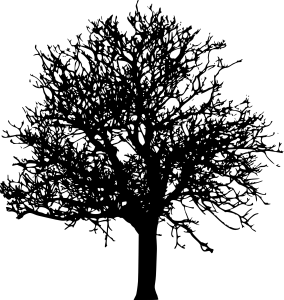
\includegraphics[width=0.4\linewidth,height=\textheight,keepaspectratio]{tree_01.png}

  \begin{enumerate}
  \def\labelenumii{(\Alph{enumii})}
  \item
    ¿Qué podemos decir sobre este gráfico?

    \begin{enumerate}
    \def\labelenumiii{\alph{enumiii}.}
    \tightlist
    \item
      Respuesta A.a
    \item
      Respuesta A.b
    \item
      Respuesta A.c
    \item
      Respuesta A.d
    \end{enumerate}
  \item
    Con respecto al código \ldots:

    \begin{enumerate}
    \def\labelenumiii{\alph{enumiii}.}
    \tightlist
    \item
      Respuesta B.a
    \item
      Respuesta B.b
    \item
      Respuesta B.c
    \item
      Respuesta B.d
    \end{enumerate}
  \end{enumerate}
\end{enumerate}

El texto sigue por aquí\ldots{}

Al escribir (\textbf{atención a las tabulaciones de 4 espacios}):

\begin{Shaded}
\begin{Highlighting}[]
\SpecialStringTok{1.  }\NormalTok{Inicio del enunciado de un ejercicio}

\NormalTok{    | Marca | valor   |}
\NormalTok{    |{-}{-}{-}{-}{-}{-}{-}|{-}{-}{-}{-}{-}{-}{-}{-}{-}|}
\NormalTok{    | A     | 0.05    |}
\NormalTok{    | B     | 0.03    |}
\NormalTok{    | C     | 0.3     |}
\NormalTok{    | D     | 0.35    |}

\NormalTok{    Para un nivel $\textbackslash{}alpha=0.02$, se concluye lo siguiente:}

\NormalTok{    a.  Respuesta 1.}

\NormalTok{    b.  Respuesta 2.}

\NormalTok{    c.  Respuesta 3.}

\NormalTok{    d.  Respuesta 4.}


\SpecialStringTok{2.  }\NormalTok{El siguiente gráfico  }

    \AlertTok{![](tree\_01.png)}\NormalTok{\{width="40\%"\}}

\NormalTok{    (A) ¿Qué podemos decir sobre este gráfico?}
    
\InformationTok{        a. Respuesta A.a}
\InformationTok{        b. Respuesta A.b}
\InformationTok{        c. Respuesta A.c}
\InformationTok{        d. Respuesta A.d}

\InformationTok{        \textless{}!{-}{-} Comentarios no se  muestran {-}{-}\textgreater{}}

\NormalTok{    (B) Con respecto al código ...:}

\InformationTok{        a. Respuesta B.a}
\InformationTok{        b. Respuesta B.b}
\InformationTok{        c. Respuesta B.c}
\InformationTok{        d. Respuesta B.d}

\InformationTok{        \textless{}!{-}{-} Comentarios no se  muestran {-}{-}\textgreater{}}
      
\NormalTok{El texto sigue por aquí...}
\end{Highlighting}
\end{Shaded}

\newpage{}

\subsection{Tablas: Grid}\label{tablas-grid}

Admiten contenido markdown en las celdas.

\subsubsection{Ejemplo 1}\label{ejemplo-1}

\begin{longtable}[]{@{}
  >{\raggedright\arraybackslash}p{(\linewidth - 4\tabcolsep) * \real{0.1667}}
  >{\raggedright\arraybackslash}p{(\linewidth - 4\tabcolsep) * \real{0.1667}}
  >{\raggedright\arraybackslash}p{(\linewidth - 4\tabcolsep) * \real{0.2917}}@{}}
\caption{Ejemplo de tabla de tipo grid.}\tabularnewline
\toprule\noalign{}
\begin{minipage}[b]{\linewidth}\raggedright
Fruit
\end{minipage} & \begin{minipage}[b]{\linewidth}\raggedright
Price
\end{minipage} & \begin{minipage}[b]{\linewidth}\raggedright
Advantages
\end{minipage} \\
\midrule\noalign{}
\endfirsthead
\toprule\noalign{}
\begin{minipage}[b]{\linewidth}\raggedright
Fruit
\end{minipage} & \begin{minipage}[b]{\linewidth}\raggedright
Price
\end{minipage} & \begin{minipage}[b]{\linewidth}\raggedright
Advantages
\end{minipage} \\
\midrule\noalign{}
\endhead
\bottomrule\noalign{}
\endlastfoot
Bananas & \$1.34 & \begin{minipage}[t]{\linewidth}\raggedright
\begin{itemize}
\tightlist
\item
  built-in wrapper
\item
  bright color
\end{itemize}
\end{minipage} \\
Oranges & \$2.10 & \begin{minipage}[t]{\linewidth}\raggedright
\begin{itemize}
\tightlist
\item
  cures scurvy
\item
  tasty
\end{itemize}
\end{minipage} \\
\end{longtable}

Al escribir:

\begin{Shaded}
\begin{Highlighting}[]
\NormalTok{+{-}{-}{-}{-}{-}{-}{-}{-}{-}{-}{-}+{-}{-}{-}{-}{-}{-}{-}{-}{-}{-}{-}+{-}{-}{-}{-}{-}{-}{-}{-}{-}{-}{-}{-}{-}{-}{-}{-}{-}{-}{-}{-}+}
\NormalTok{| Fruit     | Price     | Advantages         |}
\NormalTok{+===========+===========+====================+}
\NormalTok{| Bananas   | $1.34     | {-} built{-}in wrapper |}
\NormalTok{|           |           | {-} bright color     |}
\NormalTok{+{-}{-}{-}{-}{-}{-}{-}{-}{-}{-}{-}+{-}{-}{-}{-}{-}{-}{-}{-}{-}{-}{-}+{-}{-}{-}{-}{-}{-}{-}{-}{-}{-}{-}{-}{-}{-}{-}{-}{-}{-}{-}{-}+}
\NormalTok{| Oranges   | $2.10     | {-} cures scurvy     |}
\NormalTok{|           |           | {-} tasty            |}
\NormalTok{+{-}{-}{-}{-}{-}{-}{-}{-}{-}{-}{-}+{-}{-}{-}{-}{-}{-}{-}{-}{-}{-}{-}+{-}{-}{-}{-}{-}{-}{-}{-}{-}{-}{-}{-}{-}{-}{-}{-}{-}{-}{-}{-}+}

\NormalTok{: Ejemplo de tabla de tipo grid.}
\end{Highlighting}
\end{Shaded}

\subsubsection{Ejemplo 2: alinear
columnas}\label{ejemplo-2-alinear-columnas}

\begin{longtable}[]{@{}
  >{\raggedleft\arraybackslash}p{(\linewidth - 4\tabcolsep) * \real{0.1389}}
  >{\raggedright\arraybackslash}p{(\linewidth - 4\tabcolsep) * \real{0.1250}}
  >{\centering\arraybackslash}p{(\linewidth - 4\tabcolsep) * \real{0.2639}}@{}}
\toprule\noalign{}
\begin{minipage}[b]{\linewidth}\raggedleft
Right
\end{minipage} & \begin{minipage}[b]{\linewidth}\raggedright
Left
\end{minipage} & \begin{minipage}[b]{\linewidth}\centering
Centered
\end{minipage} \\
\midrule\noalign{}
\endhead
\bottomrule\noalign{}
\endlastfoot
Bananas & \$1.34 & built-in wrapper \\
\end{longtable}

Al escribir:

\begin{Shaded}
\begin{Highlighting}[]
\NormalTok{+{-}{-}{-}{-}{-}{-}{-}{-}{-}+{-}{-}{-}{-}{-}{-}{-}{-}+{-}{-}{-}{-}{-}{-}{-}{-}{-}{-}{-}{-}{-}{-}{-}{-}{-}{-}+}
\NormalTok{| Right   | Left   | Centered         |}
\NormalTok{+========:+:=======+:================:+}
\NormalTok{| Bananas | $1.34  | built{-}in wrapper |}
\NormalTok{+{-}{-}{-}{-}{-}{-}{-}{-}{-}+{-}{-}{-}{-}{-}{-}{-}{-}+{-}{-}{-}{-}{-}{-}{-}{-}{-}{-}{-}{-}{-}{-}{-}{-}{-}{-}+}
\end{Highlighting}
\end{Shaded}

\subsubsection{Ejemplo 3: sin cabecera}\label{ejemplo-3-sin-cabecera}

\begin{longtable}[]{@{}
  >{\raggedleft\arraybackslash}p{(\linewidth - 4\tabcolsep) * \real{0.1667}}
  >{\raggedright\arraybackslash}p{(\linewidth - 4\tabcolsep) * \real{0.1667}}
  >{\centering\arraybackslash}p{(\linewidth - 4\tabcolsep) * \real{0.1528}}@{}}
\toprule\noalign{}
\endhead
\bottomrule\noalign{}
\endlastfoot
Right & Left & Centered \\
\end{longtable}

Al escribir:

\begin{Shaded}
\begin{Highlighting}[]
\NormalTok{+{-}{-}{-}{-}{-}{-}{-}{-}{-}{-}:+:{-}{-}{-}{-}{-}{-}{-}{-}{-}{-}+:{-}{-}{-}{-}{-}{-}{-}{-}:+}
\NormalTok{| Right     | Left      | Centered |}
\NormalTok{+{-}{-}{-}{-}{-}{-}{-}{-}{-}{-}{-}+{-}{-}{-}{-}{-}{-}{-}{-}{-}{-}{-}+{-}{-}{-}{-}{-}{-}{-}{-}{-}{-}+}
\end{Highlighting}
\end{Shaded}

\subsubsection{Ejemplo 4: gráfico y otro
elemento}\label{ejemplo-4-gruxe1fico-y-otro-elemento}

\begin{longtable}[]{@{}
  >{\raggedright\arraybackslash}p{(\linewidth - 2\tabcolsep) * \real{0.2639}}
  >{\raggedright\arraybackslash}p{(\linewidth - 2\tabcolsep) * \real{0.3889}}@{}}
\toprule\noalign{}
\begin{minipage}[b]{\linewidth}\raggedright
Gráfico
\end{minipage} & \begin{minipage}[b]{\linewidth}\raggedright
Comentarios
\end{minipage} \\
\midrule\noalign{}
\endhead
\bottomrule\noalign{}
\endlastfoot
\pandocbounded{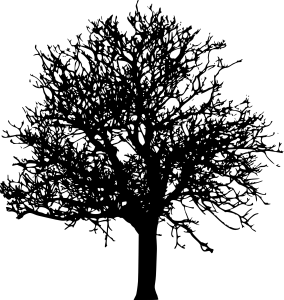
\includegraphics[keepaspectratio]{tree_01.png}} &
\begin{minipage}[t]{\linewidth}\raggedright
\begin{enumerate}
\def\labelenumi{\arabic{enumi}.}
\tightlist
\item
  Primer comentario
\item
  Segundo \textbf{comentario}
\end{enumerate}
\end{minipage} \\
\end{longtable}

O variante 1:

\begin{figure}

\begin{minipage}{0.40\linewidth}
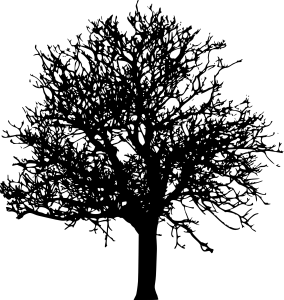
\includegraphics[width=1.04167in,height=\textheight,keepaspectratio]{tree_01.png}\end{minipage}%
%
\begin{minipage}{0.20\linewidth}
~\end{minipage}%
%
\begin{minipage}{0.40\linewidth}

\begin{enumerate}
\def\labelenumi{\arabic{enumi}.}
\tightlist
\item
  Primer comentario
\item
  Segundo \textbf{comentario}
\end{enumerate}

\end{minipage}%

\end{figure}%

O variante 2:

\begin{figure}

\begin{minipage}{0.40\linewidth}
\pandocbounded{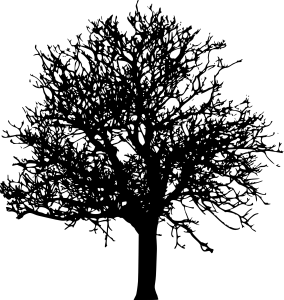
\includegraphics[keepaspectratio]{tree_01.png}}\end{minipage}%
%
\begin{minipage}{0.20\linewidth}
~\end{minipage}%
%
\begin{minipage}{0.40\linewidth}

\begin{longtable}[]{@{}lll@{}}
\caption{Segunda Tabla}\label{tbl-segundabb}\tabularnewline
\toprule\noalign{}
Col1 & Col2 & Col3 \\
\midrule\noalign{}
\endfirsthead
\toprule\noalign{}
Col1 & Col2 & Col3 \\
\midrule\noalign{}
\endhead
\bottomrule\noalign{}
\endlastfoot
A & B & C \\
E & F & G \\
A & G & G \\
\end{longtable}

\end{minipage}%

\end{figure}%

Esta variante 2 se obtiene al escribir:

\begin{Shaded}
\begin{Highlighting}[]
\NormalTok{:::: \{layout="}\CommentTok{[}\OtherTok{40,{-}20,40}\CommentTok{]}\NormalTok{" layout{-}valign="top"\}}

\AlertTok{![](tree\_01.png)}\NormalTok{\{width=80\%\}}

\NormalTok{| Col1 | Col2 | Col3 |}
\NormalTok{|{-}{-}{-}{-}{-}{-}|{-}{-}{-}{-}{-}{-}|{-}{-}{-}{-}{-}{-}|}
\NormalTok{| A    | B    | C    |}
\NormalTok{| E    | F    | G    |}
\NormalTok{| A    | G    | G    |}
\NormalTok{: Segunda Tabla \{\#tbl{-}segundabb\}}

\NormalTok{::::}
\end{Highlighting}
\end{Shaded}

\newpage{}

\subsection{Tablas a partir de cálculos con
R}\label{tablas-a-partir-de-cuxe1lculos-con-r}

\begin{Shaded}
\begin{Highlighting}[]
\FunctionTok{library}\NormalTok{(knitr)}
\end{Highlighting}
\end{Shaded}

\begin{verbatim}
Warning: package 'knitr' was built under R version 4.3.3
\end{verbatim}

\begin{Shaded}
\begin{Highlighting}[]
\FunctionTok{kable}\NormalTok{(}\FunctionTok{head}\NormalTok{(cars))}
\end{Highlighting}
\end{Shaded}

\begin{longtable}[]{@{}rr@{}}
\caption{Datos en el dataset: cars}\tabularnewline
\toprule\noalign{}
speed & dist \\
\midrule\noalign{}
\endfirsthead
\toprule\noalign{}
speed & dist \\
\midrule\noalign{}
\endhead
\bottomrule\noalign{}
\endlastfoot
4 & 2 \\
4 & 10 \\
7 & 4 \\
7 & 22 \\
8 & 16 \\
9 & 10 \\
\end{longtable}

Al escribir:

\begin{Shaded}
\begin{Highlighting}[]
\FunctionTok{library}\NormalTok{(knitr)}
\FunctionTok{kable}\NormalTok{(}\FunctionTok{head}\NormalTok{(cars))}
\end{Highlighting}
\end{Shaded}

\begin{longtable}[]{@{}rr@{}}
\caption{Datos en el dataset: cars}\tabularnewline
\toprule\noalign{}
speed & dist \\
\midrule\noalign{}
\endfirsthead
\toprule\noalign{}
speed & dist \\
\midrule\noalign{}
\endhead
\bottomrule\noalign{}
\endlastfoot
4 & 2 \\
4 & 10 \\
7 & 4 \\
7 & 22 \\
8 & 16 \\
9 & 10 \\
\end{longtable}

\subsubsection{Ejemplo 2:}\label{ejemplo-2}

\begin{Shaded}
\begin{Highlighting}[]
\FunctionTok{kable}\NormalTok{(}\FunctionTok{head}\NormalTok{(cars))}
\end{Highlighting}
\end{Shaded}

\begin{longtable}[]{@{}
  >{\raggedleft\arraybackslash}p{(\linewidth - 2\tabcolsep) * \real{0.6000}}
  >{\raggedleft\arraybackslash}p{(\linewidth - 2\tabcolsep) * \real{0.4000}}@{}}

\caption{\label{tbl-cars}Datos en el dataset: cars}

\tabularnewline

\toprule\noalign{}
\begin{minipage}[b]{\linewidth}\raggedleft
speed
\end{minipage} & \begin{minipage}[b]{\linewidth}\raggedleft
dist
\end{minipage} \\
\midrule\noalign{}
\endhead
\bottomrule\noalign{}
\endlastfoot
4 & 2 \\
4 & 10 \\
7 & 4 \\
7 & 22 \\
8 & 16 \\
9 & 10 \\

\end{longtable}

Al escribir:

\begin{Shaded}
\begin{Highlighting}[]
\FunctionTok{kable}\NormalTok{(}\FunctionTok{head}\NormalTok{(cars))}
\end{Highlighting}
\end{Shaded}

\begin{longtable}[]{@{}
  >{\raggedleft\arraybackslash}p{(\linewidth - 2\tabcolsep) * \real{0.6000}}
  >{\raggedleft\arraybackslash}p{(\linewidth - 2\tabcolsep) * \real{0.4000}}@{}}

\caption{\label{tbl-cars2}Datos en el dataset: cars}

\tabularnewline

\toprule\noalign{}
\begin{minipage}[b]{\linewidth}\raggedleft
speed
\end{minipage} & \begin{minipage}[b]{\linewidth}\raggedleft
dist
\end{minipage} \\
\midrule\noalign{}
\endhead
\bottomrule\noalign{}
\endlastfoot
4 & 2 \\
4 & 10 \\
7 & 4 \\
7 & 22 \\
8 & 16 \\
9 & 10 \\

\end{longtable}

\subsubsection{Ejemplo 3:}\label{ejemplo-3}

\begin{Shaded}
\begin{Highlighting}[]
\FunctionTok{library}\NormalTok{(knitr)}
\FunctionTok{kable}\NormalTok{(}\FunctionTok{head}\NormalTok{(cars))}
\FunctionTok{kable}\NormalTok{(}\FunctionTok{head}\NormalTok{(pressure))}
\end{Highlighting}
\end{Shaded}

\begin{table}

\caption{\label{tbl-example}Ejemplo de subtablas}

\begin{minipage}{0.50\linewidth}

\subcaption{\label{tbl-example-1}Dataset: cars}

\centering{

\begin{tabular}{rr}
\toprule
speed & dist\\
\midrule
4 & 2\\
4 & 10\\
7 & 4\\
7 & 22\\
8 & 16\\
9 & 10\\
\bottomrule
\end{tabular}

}

\end{minipage}%
%
\begin{minipage}{0.50\linewidth}

\subcaption{\label{tbl-example-2}Dataset: pressure}

\centering{

\begin{tabular}{rr}
\toprule
temperature & pressure\\
\midrule
0 & 0.0002\\
20 & 0.0012\\
40 & 0.0060\\
60 & 0.0300\\
80 & 0.0900\\
100 & 0.2700\\
\bottomrule
\end{tabular}

}

\end{minipage}%

\end{table}%

Al escribir:

\begin{Shaded}
\begin{Highlighting}[]
\FunctionTok{library}\NormalTok{(knitr)}
\FunctionTok{kable}\NormalTok{(}\FunctionTok{head}\NormalTok{(cars))}
\FunctionTok{kable}\NormalTok{(}\FunctionTok{head}\NormalTok{(pressure))}
\end{Highlighting}
\end{Shaded}

\begin{table}

\caption{\label{tbl-example2}Ejemplo de subtablas}

\begin{minipage}{0.50\linewidth}

\subcaption{\label{tbl-example2-1}Dataset: cars}

\centering{

\begin{tabular}{rr}
\toprule
speed & dist\\
\midrule
4 & 2\\
4 & 10\\
7 & 4\\
7 & 22\\
8 & 16\\
9 & 10\\
\bottomrule
\end{tabular}

}

\end{minipage}%
%
\begin{minipage}{0.50\linewidth}

\subcaption{\label{tbl-example2-2}Dataset: pressure}

\centering{

\begin{tabular}{rr}
\toprule
temperature & pressure\\
\midrule
0 & 0.0002\\
20 & 0.0012\\
40 & 0.0060\\
60 & 0.0300\\
80 & 0.0900\\
100 & 0.2700\\
\bottomrule
\end{tabular}

}

\end{minipage}%

\end{table}%

\section{Diagramas de flujo con
``mermaid''}\label{diagramas-de-flujo-con-mermaid}

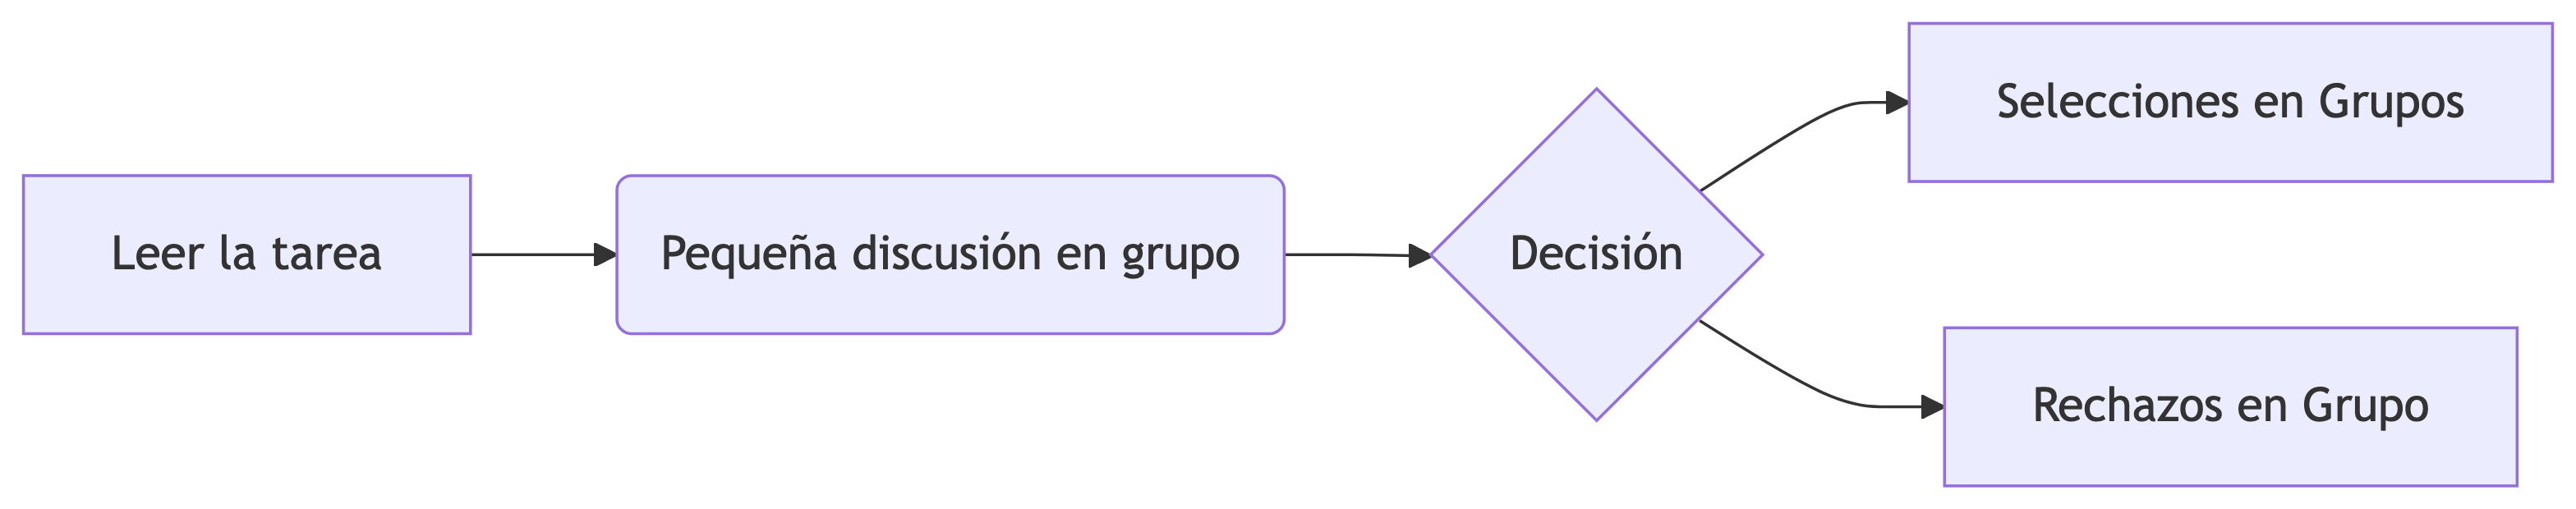
\includegraphics[width=6in,height=1.19in]{practica01c_files/figure-latex/mermaid-figure-1.png}

Al escribir:

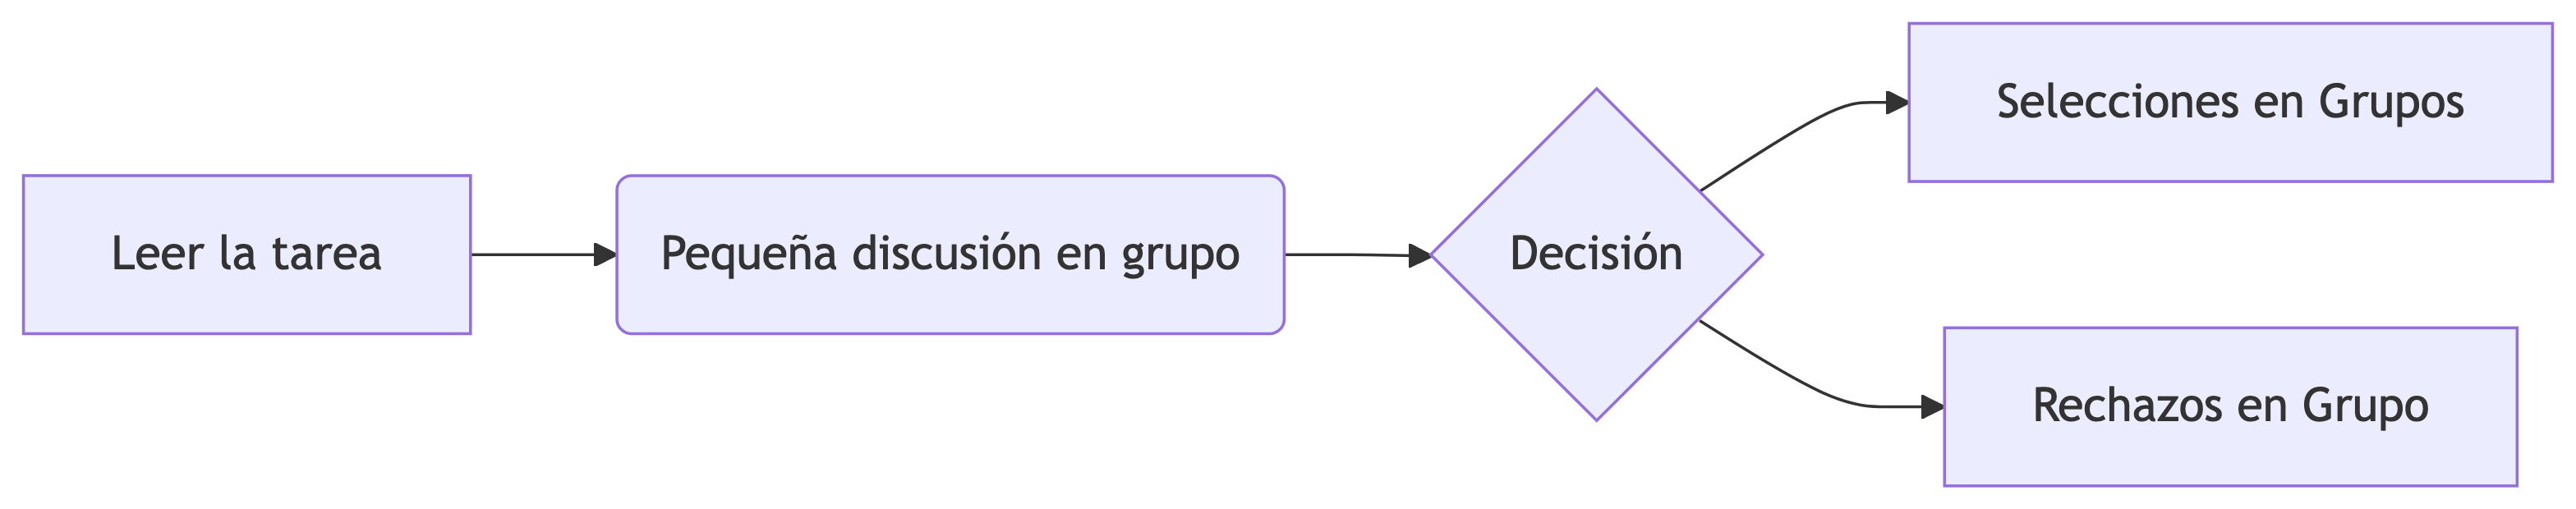
\includegraphics[width=6in,height=1.19in]{practica01c_files/figure-latex/mermaid-figure-2.png}

\section{Figuras}\label{figuras}

\begin{figure}

\centering{

This is the figure content.

\legend{This is plain text turned as LaTeX caption.}

}

\caption{\label{fig-1}This is a caption.}

\end{figure}%

\subsection{Ejemplo 2}\label{ejemplo-2-1}

\begin{figure}

\centering{

\pandocbounded{
\includegraphics[keepaspectratio]{practica01c_files/mediabag/600x400@2x.png}}

}

\caption{\label{fig-2}This is a caption.\\
\legend{This is plain text turned as LaTeX caption.}}

\end{figure}%

Al escribir:

\begin{Shaded}
\begin{Highlighting}[]
\NormalTok{::: \{\#fig{-}2\}}
\AlertTok{![](https://placehold.co/600x400@2x.png)}

\NormalTok{This is a caption.  }
\InformationTok{\textasciigrave{}\textbackslash{}legend\{This is plain text turned as LaTeX caption.\}\textasciigrave{}}\NormalTok{\{=latex\}}
\NormalTok{:::}
\end{Highlighting}
\end{Shaded}





\end{document}
